% Copyright 2022 Haute école d'ingénierie et d'architecture de Fribourg
%
% Licensed under the Apache License, Version 2.0 (the "License");
% you may not use this file except in compliance with the License.
% You may obtain a copy of the License at
%
% http://www.apache.org/licenses/LICENSE-2.0
%
% Unless required by applicable law or agreed to in writing, software
% distributed under the License is distributed on an "AS IS" BASIS,
% WITHOUT WARRANTIES OR CONDITIONS OF ANY KIND, either express or implied.
% See the License for the specific language governing permissions and
% limitations under the License.

% =============================================================================
% | HES-SO//Master - Thesis project report template                           |
% |                                                                           |
% | Originally based on the EPFL template, with many adjustments             |
% =============================================================================

% Document settings
\documentclass[a4paper,11pt,fleqn]{book}
\usepackage[utf8]{inputenc}
\usepackage[T1]{fontenc}
\usepackage[english]{babel}



% -----------------------------------------------------------------------------
% Preamble
% -----------------------------------------------------------------------------
% =============================================================================
% | Thesis metadata                                                           |
% =============================================================================

% Thesis info
\newcommand{\ThesisTitle}{GPU optimization - Celeritas}
\newcommand{\ThesisSubject}{}
\newcommand{\Orientation}{Information and communication systems (ICS) }
\newcommand{\Keywords}{}
\newcommand{\Keywordsfr}{}
\newcommand{\reportVersion}{v0.1}
\newcommand{\specificationVersion}{v1.3}

% Author
\newcommand{\AuthorFirstName}{Simon }
\newcommand{\AuthorLastName}{Barras}
\newcommand{\Author}{\AuthorFirstName \AuthorLastName}

% Advisor
\newcommand{\AdvisorFirstName}{Frédéric }
\newcommand{\AdvisorLastName}{Bapst}
\newcommand{\AdvisorSchool}{HEIA-FR}
\newcommand{\Advisor}{Prof. \AdvisorFirstName \AdvisorLastName}
\newcommand{\AdvisorTwoFirstName}{Jean }
\newcommand{\AdvisorTwoLastName}{Hennebert}
\newcommand{\AdvisorTwoSchool}{HEIA-FR}
\newcommand{\AdvisorTwo}{Prof. \AdvisorTwoFirstName \AdvisorTwoLastName}
\newcommand{\Expert}{Dr. Baptiste Wicht}

% Mendant
\newcommand{\Mendant}{\acrfull{lbl}\\ & Paolo Calafiura\\ & Julien Esseiva}

% Place (for date and place)
\newcommand{\Date}{\today}
\newcommand{\Place}{Berkeley, CA, USA}
         % your project data
% ==================
% Template settings
% ==================

% General tools
% -------------
\usepackage{etoolbox}
\usepackage{listings}

% Page style
% ----------
\usepackage[margin=3cm, left=3.5cm, right=3.5cm, twoside=false]{geometry}
\usepackage{fancyhdr}
\setlength{\headheight}{14pt}
\renewcommand{\sectionmark}[1]{\markright{\thesection\ #1}}
\pagestyle{fancy}

% Standard pages (inside chapters)
\fancyhf{}
\renewcommand{\headrulewidth}{0.4pt}
\renewcommand{\footrulewidth}{0.4pt}
\fancyhead[R]{\bfseries \nouppercase{\rightmark}}
\fancyhead[L]{\bfseries \nouppercase{\leftmark}}
\fancyfoot[L]{\Author \space - \ThesisTitle}
\fancyfoot[R]{\thepage}

% First page of chapters
\fancypagestyle{plain}{
	\fancyhf{}
	\renewcommand{\headrulewidth}{0pt}
	\fancyfoot[L]{\Author \space - \ThesisTitle}
	\fancyfoot[R]{\thepage}
}

% Imports for external PDFs
\fancypagestyle{addpagenumbersforpdfimports}{
	\fancyhead{}
	\renewcommand{\headrulewidth}{0pt}
	\fancyfoot{}
	\fancyfoot[R]{\thepage}
}

% Use empty style for page when clearing double pages
%\def\cleartoodd{%
%	\clearpage%
%	%\ifodd\value{page}\else\mbox{}\thispagestyle{empty}\newpage\fi%
%}

%\def\clearchap{%
%	\ifodd\value{page}\else\mbox{}\thispagestyle{empty}\fi%
%}

% \cleardoublepage replaced by \cleartoodd
%\let\origdoublepage\cleardoublepage
%\renewcommand{\cleardoublepage}{%
%	\cleartoodd%
%}

% Fonts
% -----

% Helvetica (Arial used in the MSE Word template)
\usepackage{helvet}
\usepackage{lmodern}
\usepackage[T1]{fontenc}


% Math
% ----
\usepackage{amsmath}  % better math

% Floats and figures
% ------------------
\usepackage{newfloat}          % floats
\usepackage[oneside]{caption}  % captions
\usepackage{subcaption}        % subcaptions
\usepackage[section]{placeins} % allows to put float barriers

% Float captions in italics, with the label in the margin
%\DeclareCaptionLabelFormat{title}{#1 #2}
%\DeclareCaptionLabelFormat{hangout}{\llap{#1 #2\hspace{5mm}}}
%\captionsetup{
%	format=hang,
%	labelformat=hangout,
%	singlelinecheck=false,
%	font={it}
%}

% Caption with a source for a figure
% TODO: improve this to use square brackets like the normal "caption"
\newcommand*{\captionsource}[3]{%
	\caption[{#1}]{%
		#2%

		\textbf{Source:} #3%
	}%
}

% Tables
% ------
\usepackage{booktabs} % much better tables
\usepackage{multirow} % allows to fuse rows
\usepackage{array}    % manipulate array
\usepackage{tabularx} % better tables

% Define new tabularx column types:
%  - R: streteched right-aligned
%  - C: stretched centered
%  - N: left aligned, specified space
\newcolumntype{R}{>{\raggedleft\arraybackslash}X}%
\newcolumntype{C}{>{\centering\arraybackslash}X}%
\newcolumntype{N}[1]{>{\raggedleft\arraybackslash}p{#1}}

% Set row height multiplicator to provide more breathing space
\renewcommand{\arraystretch}{1.3}

% Bibliography
% -------------------

% Use biber, with numeric style and no sorting (citation order)
\usepackage[
backend=biber,
style=numeric,
sorting=none,
bibencoding=auto
]{biblatex}
\addbibresource{bibliography.bib}


% Tables of contents, figures, tables and listings
% ------------------------------------------------
\usepackage{tocloft}
\newlistof{listing}{lol}{List of Listings}
\setcounter{tocdepth}{1} % Depth to 'section'
\setlength{\cftfigindent}{0pt}  % remove indentation from figures in lof
\setlength{\cftfignumwidth}{1cm}
\setlength{\cfttabindent}{0pt}  % remove indentation from tables in lot
\setlength{\cfttabnumwidth}{1cm}
\setlength{\cftlistingindent}{0pt}
\setlength{\cftlistingnumwidth}{1cm}

% Mini tables of contents
% -----------------------
\usepackage{minitoc}

% no "Contents" title
\mtcsettitle{minitoc}{Contents}

% Layout
\setlength{\mtcindent}{-0.5em}
\mtcsetoffset{minitoc}{-1em}

% Spacing above and below table
\mtcsetfeature{minitoc}{before}{\vspace{0.5cm}}
\mtcsetfeature{minitoc}{after}{\vspace{-0.25cm}}
\renewcommand{\mtifont}{\sffamily\bfseries\large}

% Colors & graphics
% -----------------
\usepackage[table]{xcolor}    % colors
\usepackage[pdftex]{graphicx} % graphics importing
\graphicspath{{02-main/figures/}}
\definecolor{gray80}{gray}{0.80}


% Code and syntax highlighting
% ----------------------------
\usepackage[newfloat]{minted}   % code highlighting
\newenvironment{code}{\captionsetup{type=listing}}{}

% Typography
% ----------
\usepackage{csquotes}                    % paragraph indentation and spacing
\usepackage[defaultlines=3,all]{nowidow} % avoid widows and orphans
\usepackage{microtype}                   % typographic improvements
\usepackage{parskip}                     % No indent and auto-space between paragraphs
\usepackage[super]{nth}
\usepackage{amsmath}

\usepackage{paralist}
\usepackage{enumitem}
\setlist{after=\vspace{\baselineskip}}

% Section and chapters headings
% -----------------------------
\usepackage[explicit]{titlesec} % titles formatting
%\usepackage{titletoc} % titles formatting in ToC etc
%\usepackage{sectsty}  % sectioning commands

% -- Chapters --
% Remove "Chapter N" and use a sans-serif font

% Set layout lengths
\setlength{\headheight}{8mm}
\setlength{\footskip}{1.5cm}
\addtolength{\textheight}{-.5cm}

\titlespacing{\chapter}{-5mm}{-10mm}{3mm}
\titlespacing{\section}{-5mm}{3mm}{2mm}
\titlespacing{\subsection}{-5mm}{2mm}{2mm}
\titlespacing{\subsubsection}{-5mm}{2mm}{1mm}


%\titleformat{\chapter}[block]
%{\Huge}
%{\thechapter\hspace{12pt}\textcolor{gray80}{|}\hspace{12pt}}
%{0pt}
%{\Huge\bfseries}

\titleformat{\chapter}{\Huge\bfseries}{\llap{\thechapter\hspace{12pt}\textcolor{gray80}{|}}}{0mm}{%
	\hfill\begin{minipage}[t]{\dimexpr\textwidth}\raggedright#1\end{minipage}%
}
\titleformat{\section}{\Large\bfseries}{\llap{\thesection}}{0mm}{%
	\hfill\begin{minipage}[t]{\dimexpr\textwidth}\raggedright#1\end{minipage}%
}
\titleformat{\subsection}{\large \bfseries}{\llap{\thesubsection}}{0mm}{%
	\hfill\begin{minipage}[t]{\dimexpr\textwidth}\raggedright#1\end{minipage}%
}
\titleformat{\subsubsection}{\bfseries}{\llap{\thesubsubsection}}{0mm}{%
	\hfill\begin{minipage}[t]{\dimexpr\textwidth}\raggedright#1\end{minipage}%
}

% Misc
% ------
\usepackage{lipsum}    % filler text
\usepackage{blindtext} % random text
\usepackage{lscape}    % easy landscape pages
\usepackage{pdflscape} % landscape pages for PDFs

% Allow email typesetting
\newcommand{\email}[1]{%
	\href{mailto:#1}{\textit{#1}}%
}

% References
% -----------
\usepackage{url}

% pdf metadata
\usepackage[
	pdfauthor={\Author},
	pdftitle={\ThesisTitle},
	pdfsubject={\ThesisSubject},
	pdfkeywords={\Keywords}
	pdfduplex=DuplexFlipLongEdge]{hyperref}

% Hyperlinks
\hypersetup{
	colorlinks=true,
	linkcolor=black,
	citecolor=black,
	filecolor=black,
	urlcolor=black,
}
\providecommand*{\listingautorefname}{Listing}


% % Glossary
% % --------
%\usepackage[xindy, toc, nonumberlist]{glossaries}
\usepackage[acronym]{glossaries}
\makeglossaries
\newacronym{heia}{HEIA-FR}{Haute Ecole d'Ingénierie et d'Architecture de Fribourg}

\newacronym{os}{OS}{Operating System}

\newacronym{gpu}{GPU}{Graphics Processing Unit}

\newacronym{cpu}{CPU}{Central Processing Unit}

\newacronym{cuda}{CUDA}{Compute Unified Device Architecture}

\newacronym{lbl}{LBNL}{Lawrence Berkeley National Laboratory}

\newacronym{ornl}{ORNL}{Oak Ridge National Laboratory}

\newacronym{anl}{ANL}{Argonne National Laboratory}

\newacronym{fnal}{FNAL}{Fermi National Accelerator Laboratory}

\newacronym{bnl}{BNL}{Brookhaven National Laboratory}

\newacronym{cern}{CERN}{European Organization for Nuclear Research}

\newacronym{lhc}{LHC}{Large Hadron Collider}

\newacronym{doe}{DOE}{Department of Energy}

\newacronym{smart}{SMART}{Specific, Measurable, Achievable, Relevant, Time-bound}

\newacronym{hpc}{HPC}{High Performance Computing}

\newacronym{nersc}{NERSC}{National Energy Research Scientific Computing Center}

\newacronym{atlas}{ATLAS}{A Toroidal LHC ApparatuS}

\newacronym{cms}{CMS}{Compact Muon Solenoid}

\newacronym{hep}{HEP}{High Energy Physics}

\newacronym{rkdp}{RKDP}{Runge Kutta Dormand Prince}

\newacronym{simd}{SIMD}{Single Instruction Multiple Data}

\newacronym{sisd}{SISD}{Single Instruction Single Data}

\newacronym{sm}{SM}{Streaming Multiprocessor}

\newacronym{sdk}{SDK}{Software Development Kit}

\newacronym{api}{API}{Application Programming Interface}

\newacronym{simt}{SIMT}{Single Instruction Multiple Thread}



\usepackage{tabularray}    % template settings
% ===========================================
% = Codestyles for minted syntax highlighting
% ===========================================


% How to use (replace 'java' with language name):
% - code blocks:
%     \begin{javacode}
%     CODE
%     \end{javacode}
% - files:
%     full: \javafile{PATH}
%     extract: \javafile[startline=x, endline=y]{PATH}

% c#
\newminted{csharp}{frame=single, framesep=6pt, breaklines=true, fontsize=\scriptsize}
\newmintedfile{csharp}{frame=single, framesep=6pt, breaklines=true,
fontsize=\scriptsize}

% Java
\newminted{java}{frame=single, framesep=6pt, breaklines=true, fontsize=\scriptsize}
\newmintedfile{java}{frame=single, framesep=6pt, breaklines=true,
fontsize=\scriptsize}

% JavaScript
\newminted{js}{frame=single, framesep=6pt, breaklines=true, fontsize=\scriptsize}
\newmintedfile{js}{frame=single, framesep=6pt, breaklines=true, fontsize=\scriptsize}

% Scala
\newminted{scala}{frame=single, framesep=6pt, breaklines=true, fontsize=\scriptsize}
\newmintedfile{scala}{frame=single, framesep=6pt, breaklines=true,
	fontsize=\scriptsize}

% Clojure
\newminted{clojure}{frame=single, framesep=6pt, breaklines=true, fontsize=\scriptsize}
\newmintedfile{clojure}{frame=single, framesep=6pt, breaklines=true,
	fontsize=\scriptsize}

% Python
\newminted{python}{frame=single, framesep=6pt, breaklines=true, fontsize=\scriptsize}
\newmintedfile{python}{frame=single, framesep=6pt, breaklines=true, fontsize=\scriptsize}

% Sql
\newminted{sql}{frame=single, framesep=6pt, breaklines=true, fontsize=\scriptsize}
\newmintedfile{sql}{frame=single, framesep=6pt, breaklines=true, fontsize=\scriptsize}

% Json
\newminted{json}{frame=single, framesep=6pt, breaklines=true, fontsize=\scriptsize}
\newmintedfile{json}{frame=single, framesep=6pt, breaklines=true,
	fontsize=\scriptsize}

% Yaml
\newminted{yaml}{frame=single, framesep=6pt, breaklines=true,
fontsize=\scriptsize}
\newmintedfile{yaml}{frame=single, framesep=6pt, breaklines=true,
	fontsize=\scriptsize}

% Plain text
\newminted{text}{frame=single, framesep=6pt, breaklines=true, breakanywhere, fontsize=\scriptsize}
\newmintedfile{text}{frame=single, framesep=6pt, breaklines=true, breakanywhere, fontsize=\scriptsize}

% Bash
\newminted{bash}{frame=single, framesep=6pt, breaklines=true, fontsize=\scriptsize}
\newmintedfile{bash}{frame=single, framesep=6pt, breaklines=true, fontsize=\scriptsize}
       % code styles for minted
% ========================
% = TODO: Document
% ========================

% Marc's font stack
\usepackage{cmbright}       % Sans serif
\usepackage{sourcecodepro}  % Monospace
\usepackage{float}
\renewcommand{\familydefault}{\sfdefault}

\newcommand{\todo}[1]{\textcolor{red}{\textbf{TODO:} #1}}

\newcommand{\image}[4]{
    \begin{figure}[ht]
        \centering
        \includegraphics[width=#1\textwidth]{#2}
        \caption{#3}
        \label{#4}
    \end{figure}
}
  % your custom packages etc

% Glossary
% --------

% \usepackage[toc]{glossaries}
% \makeglossaries
% \newacronym{heia}{HEIA-FR}{Haute Ecole d'Ingénierie et d'Architecture de Fribourg}

\newacronym{os}{OS}{Operating System}

\newacronym{gpu}{GPU}{Graphics Processing Unit}

\newacronym{cpu}{CPU}{Central Processing Unit}

\newacronym{cuda}{CUDA}{Compute Unified Device Architecture}

\newacronym{lbl}{LBNL}{Lawrence Berkeley National Laboratory}

\newacronym{ornl}{ORNL}{Oak Ridge National Laboratory}

\newacronym{anl}{ANL}{Argonne National Laboratory}

\newacronym{fnal}{FNAL}{Fermi National Accelerator Laboratory}

\newacronym{bnl}{BNL}{Brookhaven National Laboratory}

\newacronym{cern}{CERN}{European Organization for Nuclear Research}

\newacronym{lhc}{LHC}{Large Hadron Collider}

\newacronym{doe}{DOE}{Department of Energy}

\newacronym{smart}{SMART}{Specific, Measurable, Achievable, Relevant, Time-bound}

\newacronym{hpc}{HPC}{High Performance Computing}

\newacronym{nersc}{NERSC}{National Energy Research Scientific Computing Center}

\newacronym{atlas}{ATLAS}{A Toroidal LHC ApparatuS}

\newacronym{cms}{CMS}{Compact Muon Solenoid}

\newacronym{hep}{HEP}{High Energy Physics}

\newacronym{rkdp}{RKDP}{Runge Kutta Dormand Prince}

\newacronym{simd}{SIMD}{Single Instruction Multiple Data}

\newacronym{sisd}{SISD}{Single Instruction Single Data}

\newacronym{sm}{SM}{Streaming Multiprocessor}

\newacronym{sdk}{SDK}{Software Development Kit}

\newacronym{api}{API}{Application Programming Interface}

\newacronym{simt}{SIMT}{Single Instruction Multiple Thread}


\begin{document}


% -----------------------------------------------------------------------------
% Front matter
% -----------------------------------------------------------------------------
\frontmatter

\dominitoc

% ==========================================================================
% = HES-SO Master thesis title page (modeled after Word template, 2016-2017)
% ==========================================================================

\begin{titlepage}
\newgeometry{margin=2cm}
{\fontfamily{phv}\fontseries{mc}\selectfont
    \begin{center}
	    
\includegraphics[width=0.95\textwidth]{05-resources/img/heiafr_logo}
		~\\[1.5cm]
		% Title
		{
			\Huge
			PS6 - \ThesisTitle\\Project report \\[0.5cm]
			\large Computer science and Communication System (ISC), 2022-2023\\[2cm]
		}
		
\includegraphics[width=0.35\textwidth]{05-resources/img/logo.png}
		~\\[2cm]
		% Info
		{
			\begin{center}
			\begin{tabularx}{\textwidth} { %tableau pour créer 2 colonnes
				>{\raggedright\arraybackslash}X
				>{\raggedright\arraybackslash}X  }
					 \textbf{Student} & \Author\\
					 & \\
					 \textbf{Supervisors} & \Advisor \space - \AdvisorSchool \\ & \AdvisorTwo \space - \AdvisorTwoSchool \\
					 & \\
					 \textbf{Customer} & \Mendant\\
			\end{tabularx}
			\end{center}
			~\\[1.5cm]
		}
%		{
%			\large
%			External expert: \\
%			\Expert
%		}

        % {
        % Le code de ce projet est disponible en open source avec l'accord de tous ses
        % participants.
        % }
		\vfill



		% Bottom of the page
	    {\reportVersion}\\
		{\large \Place, \Date}

	\end{center}
}
\restoregeometry
\end{titlepage}






% Page for student info and signatures
% \cleardoublepage
% \chapter*{Information about this report}

\vspace{\fill}

\textbf{Contact information}

\begin{tabularx}{\textwidth}{N{2.5cm}X}
	Author:	 & \AuthorFirstName \AuthorLastName \\
	& MSE Student \\
	& HES-SO//Master \\
	& Switzerland \\
	Email: & \email{\AuthorEmail}
\end{tabularx}

\vspace{\fill}

\textbf{Declaration of honor}

{\renewcommand{\arraystretch}{2}
\begin{tabularx}{\textwidth}{N{2.5cm}X}
	& I, undersigned, \Author, hereby declare that the work submitted is
	the result of a personal work. I certify that I have not resorted to
	plagiarism or other forms of fraud. All sources of information used and the
	author quotes were clearly mentioned. \\
	Place, date: & \underline{\hspace{7cm}} \\
	Signature: & \underline{\hspace{7cm}}
\end{tabularx}
}

\vspace{\fill}

%\textbf{Validation}

%Accepted by the HES-SO//Master (Switzerland, Lausanne) on a proposal from:
Accepté par la HES SO//Master (Suisse, Lausanne) sur proposition de

\vspace{0.5cm}

\Advisor %, Thesis project advisor

%\Expert, \ExpertLab, Main expert

\vspace{1cm}

Lieu, date: \underline{\hspace{8cm}}

\vspace{3cm}

{ \renewcommand{\arraystretch}{1.5}
\begin{tabularx}{\textwidth}{X X}
	\Advisor  & \Dean\\
	Advisor   & Dean, HES-SO//Master\\
\end{tabularx}
}

% Acknowledgments (your dedication etc)
% \cleardoublepage
% \chapter*{Acknowledgments}
\markboth{Acknowledgements}{Acknowledgements}
\addcontentsline{toc}{chapter}{Acknowledgements}

% -- Your text goes here --
\lipsum[1-2]



% Preface (to be written by someone else)
% \cleardoublepage
% \chapter*{Preface}
\markboth{Preface}{Preface}
\addcontentsline{toc}{chapter}{Preface}
% put your text here
A preface is not mandatory. It would typically be written by some other person (eg your thesis director).

\lipsum[1-2]

\bigskip

\noindent\textit{Lausanne, 12 Mars 2011}
\hfill T.~D.


% French + English abstracts
%\cleardoublepage
%% English abstract
\chapter*{Abstract}
%\markboth{Abstract}{Abstract}
\addcontentsline{toc}{chapter}{Abstract} % adds an entry to the table of contents

\vskip0.5cm
\textbf{Key words: }
\Keywords


% French abstract
% \cleardoublepage
% \begin{otherlanguage}{french}
% \chapter*{Résumé}
% %\markboth{Résumé}{Résumé}

% \lipsum[1-2]

% \vskip0.5cm
% \textbf{Mots clés:}
% \Keywordsfr
% \end{otherlanguage}



% Table of contents
\phantomsection
\chapter{Executive summary}
\label{ch:report-executive-summary}

\todo{Write something here}

\chapter{Version history}
\label{chap:report-versions}

\begin{tabular}{|m{0.15\textwidth}|m{0.7\textwidth}|m{0.15\textwidth}|}
 \hline
 \textbf{Version} & \textbf{Changes} & \textbf{Date} \\ [0.5ex]
 \hline
 0.1 & First version of the analysis. Adding the information about the microdispenser, the microcontroller and the programming language & 21.03.2023  \\
\hline
 1.0 & Finish the report & 18.05.2023  \\
\hline
\end{tabular}
\addcontentsline{toc}{chapter}{Contents}
\setcounter{tocdepth}{3}
\tableofcontents

% List of tables
% \cleardoublepage
% \phantomsection
% \addcontentsline{toc}{chapter}{Liste des tables}
% \listoftables

% List of listings
% \cleardoublepage
% \phantomsection
% \addcontentsline{toc}{chapter}{List of Listings}
% \listoflistings

% Restore paragraphs
\setlength{\parskip}{1em}

% Bold fonts for sections in minitoc
\renewcommand{\cftsecfont}{\sffamily\bfseries}
\renewcommand{\cftsecleader}{\sffamily\bfseries\cftdotfill{\cftdotsep}}
\renewcommand{\cftsecpagefont}{\sffamily\bfseries}


% -----------------------------------------------------------------------------
% Main matter
% -----------------------------------------------------------------------------
\mainmatter

% Chapters
\setcounter{mtc}{4} % Help minitoc skip the front matter chapters
\chapter{Introduction}
\label{ch:introduction}

This Bachelor thesis is done by Simon Barras and supervised by Frederic Bapst
and Jean Hennebert.
The customer Paolo Calafiura is a physicist and computer scientist at the \acrfull{lbl}.
To do this project, I am moving to Berkeley, California, for ten weeks.
The goal is to explore a way to improve the performance of the project Celeritas,
which is a particle physics simulation software accelerated by \acrshort{gpu}s.

The two main customers are \acrshort{cms} and \acrshort{atlas}, two experiments
are made at the \acrfull{cern} with the \acrfull{lhc} and run
their simulation with Geant4.
They are both using Geant4 and they have not committed to using Celeritas
beyond an initial evaluation.
Detector simulation is used to validate and calibrate the algorithms used to
estimate the properties of the primary particles from the observed detector data.
The main goal of the thesis will be to optimize a GPU-accelerated version of
the Prince Dormand algorithm~\cite{princeDormand}, a
Runge-Kutta solver~\cite{Runge-Kutta-methods} for the differential equations
governing the trajectory of particles in a non-uniform magnetic field.
This work will improve the project Celeritas~\cite{Celeritas-Project} which may
replace Geant4~\cite{geant4} in the future.

The \acrshort{atlas} experiment tracks the path of particles in the detector and
produces coordinates points where particles traverse the sensors.
Figure \ref{fig:introduction:particles:tracking} represents this experiment.
\begin{figure}[ht]
    \centering
    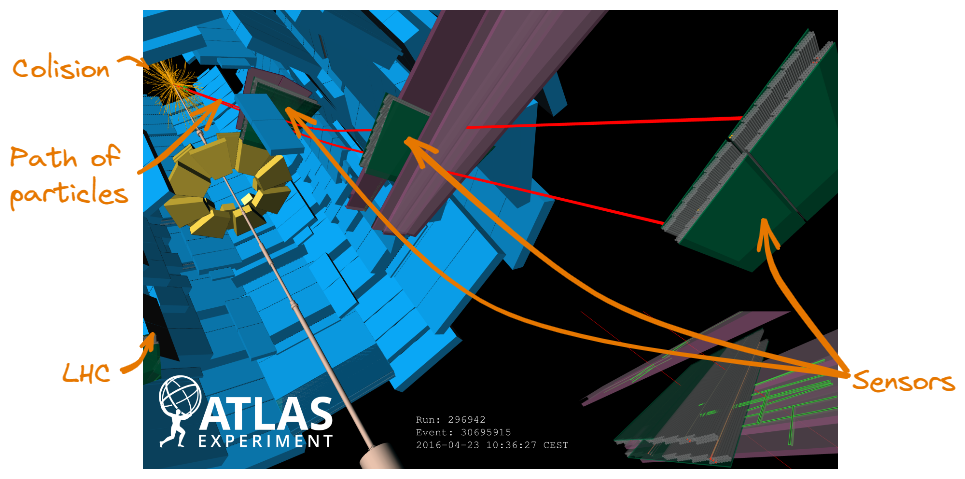
\includegraphics[width=0.85\textwidth]{05-resources/img/spec/experiment-atlas.excalidraw.png}
    \caption{ATLAS experiment at CERN~\cite{atlas-experiment}}
    \label{fig:introduction:particles:tracking}
\end{figure}

\section{Lawrence Berkeley National Laboratory}
\label{ch:introduction:lbl}

The \acrfull{lbl} is a national laboratory in Berkeley, California.
It is managed and operated by the University of California for the \acrfull{doe}.
The lab is situated in the hills of Berkeley and it is composed of many buildings
and has a beautiful view of the San Francisco Bay (see Fig.\ref{fig:introduction:lbl:view}).
This laboratory is mentioned in the recently released movie by Christopher Nolan,
"Oppenheimer".

\begin{figure}[ht]
    \centering
    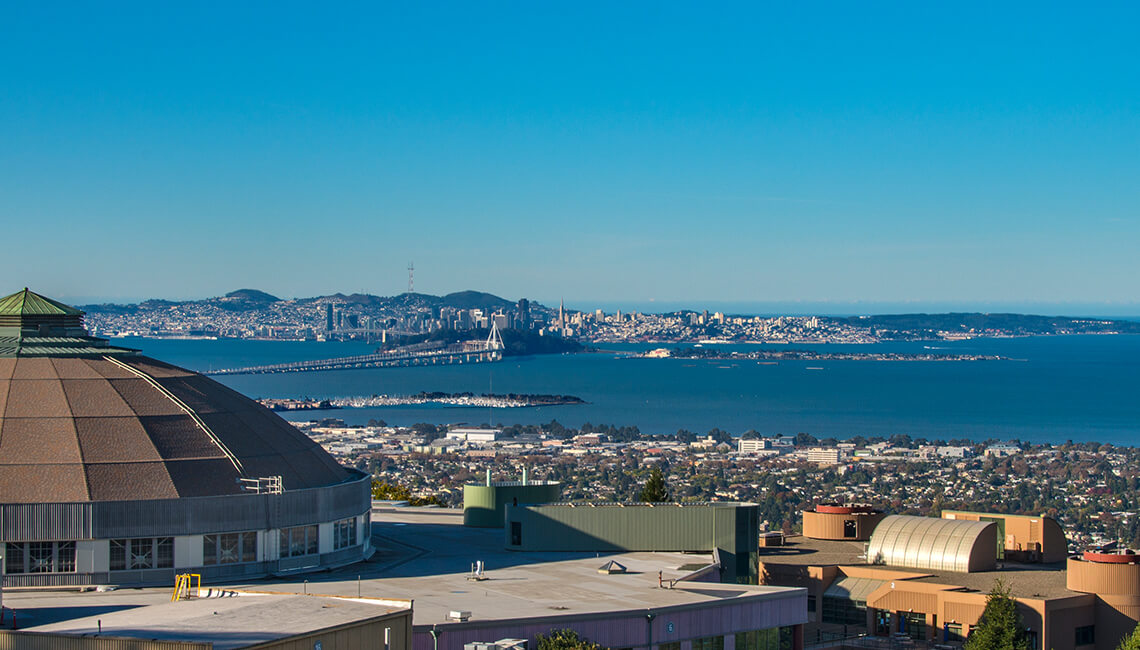
\includegraphics[width=0.8\textwidth]{05-resources/img/spec/lab-view.jpg}
    \caption{Lawrence Berkeley National Laboratory}
    \label{fig:introduction:lbl:view}
\end{figure}


\section{The objectives}
\label{ch:introduction:objectives}

Celeritas is already accelerated by \acrshort{gpu}s, however, the team wants to
improve the performance.
In the current version of the code, each particle track is processed in parallel
by one GPU thread, with no collaboration between threads.
GPU profiling of the code shows that execution time is dominated by two kernels.
The first one is handled by the interaction with the detector geometry to know
where, in 3D space, the particle is situated and during the profiling, the
library used is vecGeom~\cite{VecGeom}.
The second kernel, which will be the focus of this Bachelor thesis project, is
the computation of a differential equation using Dormand-Prince~\cite{princeDormand}.

However, the thesis can be a success even if the project doesn't meet the improvement.
This is because we don't yet know whether thread synchronization will be more
time-consuming than the original version.
In addition, the kernel launch in Celeritas have to be changed, and this
could take up a considerable amount of optimization time.
For the Bachelor thesis, it is sufficient to have a proof of concept that
demonstrates if the enhancement is effective and deserves to be integrated.
To measure the changes done during the internship, the profiler must be run
before and after each step of the project.
The mandatory requirements are described in the following section.

\subsection{Learn GPU programming}
\label{ch:introduction:objectives:learn-gpu-programming}

Before starting to work on the project, some things need to be learned and the goal here is to learn a new way of programming.
To conclude this goal, no code will be produced except for exercises, but the important notions of \acrshort{gpu} programming with CUDA will be synthesized using cheat sheets.
To take advantage of the delay between the beginning of the Bachelor thesis and the beginning of the \acrshort{lbl} internship, this step will be done during this time.


\subsection{Understand the project}
\label{ch:introduction:objectives:understand-the-project}

To be able to improve the performance of the code, the first step is to understand the project and it's always better to understand the background: why it is needed, who will use it and which paradigm and tools are used.

To measure the performance gained, it is necessary to know where the project is at each step.
To take a snapshot of the performance, a profiler can be run and this includes that we can compile and launch the project.
This step will be done at the beginning of the project on-site.


\subsection{Improve the performance}
\label{ch:introduction:objectives:improve-the-performance}

The main goal of the project is to improve the performance of the implementation of Dormand-Prince method~\cite{princeDormand}.
This last mandatory requirement is the core of the thesis and the most important part of the project and it will require the knowledge gained in the first two steps to improve the performance.

To conclude this step, the code must compile, pass the unit test, and a profiler must be run to show the difference between the new and the legacy implementation of the DormandPrince method.
To achieve this goal, the profiles must show an improvement, but this could meet some difficulties to be realized and integrated into the project.
In all cases, the failure of this goal doesn't mean the failure of the thesis if the documentation is correctly done and explains the results obtained and how is it possible or not to continue to this path.
This step will be done after the first two steps and it will take the whole time left.

\section{Optional requirements}
\label{ch:introduction:optional-requirements}

These optional goals are good additions to the project but they are not
require to have a concrete result.

The first one is to have a portable performance.
The purpose of Celeritas is to be run on all kinds of \acrshort{gpu} and even on machines with just a \acrshort{cpu}.
During the optimization, the improvement will be checked on the Perlmutter~\cite{Perlmutter} which uses Nvidia A100 with the architecture Ampere~\cite{ampere} and some improvement can be only effective to this kind of \acrshort{gpu}.
This goal is here to check if the improvement has a positive effect on other architectures and if it is not, to find a way to do that.
To begin this step, the main goal needs to be finished.

The second optional objective is to do another performance improvement.
If the performance of the Runge-Kutta method~\cite{Runge-Kutta-methods} is improved, another optimization can be done.
This part goal will be discussed further in the project with the supervisors and the customers and it will be managed like the last mandatory goal.
This step can be done multiple times if there is enough time.

\chapter{Analyze}
\label{ch:analyze}

During this chapter, the project is analyzed to understand the context, the
goals and challenges.
This project is focused on the optimization of the particle's tracking using
\acrshort{gpu}s.
The \acrshort{gpu}'s programming is something totally new for a bachelor's
student at the \acrshort{heia}.
Celeritas is a project that is actively developed and it requires time to
understand the code and the architecture.


\section{GPU}
\label{ch:analyze:gpu}

The \acrfull{gpu} is a processor that is specialized in parallel computing.
It is known by the gamer community because it is used to render the graphics of
the games and a good graphic card increases the frame per second displayed.
However, in the professional world, the \acrshort{gpu} are becoming more and
more popular because they are more efficient than the \acrshort{cpu} for
parallel computing and managing a large amount of data.


\subsection{Use cases}
\label{ch:analyze:gpu:use-cases}

In most of the case, \acrshort{cpu}s are more efficient than \acrshort{gpu}s
that is why they are a mandatory component of a computer.
\acrshort{cpu}s have a high frequency and they are optimized to execute one
task at a time with a high efficiency.
In the other hand, \acrshort{gpu}s have a lower frequency and they are optimized
to execute multiple tasks at the same time.

To understand, imagine John wants to eat dinner with his 5 kids and they have to
cook something and dress the table.
Cooking is a task that must be done sequentially and require some skills and
efficiency to be done quickly.
Dressing the table is a task where the skills don't affect the time but the
number of hands does.
This task can be done by the kids when everyone is putting something on the table.
In our case, John is the \acrshort{cpu} and the kids are the \acrshort{gpu}s.

The \acrshort{gpu}s are used when the number of workers is more important than
the efficiency of the worker like computing the pixels of an image or the
particles of a simulation.




\subsection{Architecture}
\label{ch:analyze:gpu:architecture}

The table \ref{tab:analyze:gpu:architecture:instruction-data} shows the
different types of processors.
The capabilities to work with one or multiple data and instructions are defined
by the architecture of the processor.

\begin{table}[ht]
    \centering
    \begin{tabular}{l|l|l|}
                          & Single data & Multiple data \\ \hline
    Single instruction    & SISD        & \textbf{SIMD}  \\ \hline
    Multiple instructions & MISD        & MIMD           \\ \hline
    \end{tabular}
    \caption{Different types of processors working with one or multiple data and instructions}
    \label{tab:analyze:gpu:architecture:instruction-data}
\end{table}

The \acrshort{gpu} is a \acrshort{simd} processor and the \acrshort{cpu} is a
\acrshort{sisd} processor.
The table \ref{tab:analyze:gpu:architecture:instruction-data} does not show the
frequency of the processor that is an important factor for the performance.
This explains why the \acrshort{cpu} is more efficient than the \acrshort{gpu}
for most of the cases.

To deal with the \acrshort{simd} architecture, the \acrshort{gpu} executed
physically the same instruction on multiple data using multiple threads as shown
on the figure \ref{fig:analyze:gpu:architecture:smid}.

\image{0.35}{05-resources/img/analyze/simd.png}
{SIMD physically executed}
{fig:analyze:gpu:architecture:smid}

The \acrshort{gpu} is composed of multiple \acrfull{sm} that are composed of
multiple \acrfull{cuda} cores.
The \acrshort{cuda} cores are the processors that execute the instructions.
The \acrshort{sm} is the unit that manages the threads and the memory.
\ref{fig:analyze:gpu:architecture:sm} shows the architecture of a \acrshort{sm}.

\image{0.65}{05-resources/img/analyze/sm.png}
{\acrshort{sm} architecture~\cite{nvidia-a100-architecture}}
{fig:analyze:gpu:architecture:sm}

The figure \ref{fig:analyze:gpu:architecture:sm} introduces the warp that is a
group of 32 threads that are executed in parallel.
The threads of a warp are linked together and they have to wait for the others
to finish their instructions.


\section{CUDA}
\label{ch:analyze:cuda}

\acrfull{cuda} is a parallel computing platform and programming model developed
by Nvidia.
It allows developers to use the \acrshort{gpu} to execute code written in C++, C, Fortran
and Python.
The \acrshort{cuda} platform is come with a \acrshort{sdk} that provides
libraries, debugging and profiling tools.

To develop with \acrshort{cuda}, the \acrshort{sdk} must be installed and all
the examples in this report are with C++ because it is the language used in the
project.

\subsection{Basis}
\label{ch:analyze:cuda:basis}

The code that runs on a \acrshort{gpu} is in a function called "kernel" and it
is executed by every thread.
Those kernels are defined with the keyword \texttt{\_\_global\_\_} and they are called
with the function \texttt{kernel\_name<<<number\_of\_blocks, number\_of\_threads>>>()}.
The code \ref{code:analyze:cuda:develop:basis:kernel} shows a basic kernel
launch with 2 blocks and 3 threads that say that the kernel code will be
executed 6 times.

\begin{code}
    \captionof{listing}{Basic kernel example}
    \label{code:analyze:cuda:basis:kernel}
    \begin{minted}{C++}
__global__ void kernel_name() {
    // Code executed on the device
}

int main() {
    // Code executed on the host
    kernel_name<<<2, 3>>>();
    return 0;
}
    \end{minted}
\end{code}

\subsection{Memory}
\label{ch:analyze:cuda:memory}

As the \acrshort{gpu} is a separate processor, it has its own memory system.
As a developer we have to manage three different spaces where data can be stored:
\begin{itemize}
    \item Host memory (RAM)
    \item Device memory (DRAM)
    \item Shared memory
\end{itemize}

Every space becomes with their properties and use the right one is important to
have a good performance.
The figure \ref{fig:analyze:cuda:memory:architecture} shows the physical
organization of the memory on a \acrshort{gpu}.

\image{1}{05-resources/img/analyze/gpu-memory.png}
{Physical memory organization on a \acrshort{gpu}~\cite{cuda-training}}
{fig:analyze:cuda:memory:architecture}


\subsubsection{Host memory}
\label{ch:analyze:cuda:memory:host}

Memory allocated on the host is the memory we use every day but it is not
accessible by the \acrshort{gpu}.
Even if a program is using the \acrshort{gpu}, it still needs to use the host
memory.

\subsubsection{Device memory}
\label{ch:analyze:cuda:memory:device}

The device memory is the memory that is used by the \acrshort{gpu} to execute
the kernel and it is comparable to a heap memory.
This place contains the local variables of a thread, the global variables and
the constant memory.
This memory is accessible by all the threads and the data could be loaded and saved
from the host.

The arguments passed to a kernel can only be 64 bytes long so the object must be
passed by reference and the value must be copied in the device memory.
To get the result, the data must be copied back to the host memory.
The code \ref{code:analyze:cuda:memory:device:copy-read} to launch a kernel
with objects and integers as arguments.
As the kernel isn't executed on the host, the return keyword can't be used to
get the result of the kernel so the result must be copied back to the host
using the same mechanism as the arguments.

\begin{code}
    \captionof{listing}{Load ang read data from the device memory}
    \label{code:analyze:cuda:memory:device:copy-read}
    \begin{minted}{C++}
__global__ void kernel_name(ObjectType1 *input1,
                            int input2,
                            ObjectType2 *output) {
    ObjectType3 local_variable;
    output[threadIdx.x] = ObjectType2(input1[threadIdx.x] + input2);
}

int main() {
    // Instantiate the variables
    ObjectType1 *h_input1, *d_input1;
    ObjectType2 *h_output, *d_output;

    // Setting the values
    h_input1 = new ObjectType1[100];
    for (int i = 0; i < 100; i++) {
        h_input1[i] = ObjectType1(i);
    }
    h_output = new ObjectType2[100];
    int input2 = 5;

    // Allocate the memory on the device
    cudaMalloc(&d_input1, 100 * sizeof(ObjectType1));
    cudaMalloc(&d_output, 100 * sizeof(ObjectType2));

    // Copy the data from the host to the device
    cudaMemcpy(d_input1,
               h_input1,
               100 * sizeof(ObjectType1),
               cudaMemcpyHostToDevice);

    // Launch the kernel
    kernel_name<<<1, 100>>>(d_input1, input2, d_output);

    // Copy the data from the device to the host
    cudaMemcpy(h_output,
               d_output,
               100 * sizeof(ObjectType2),
               cudaMemcpyDeviceToHost);

    // Free the memory
    cudaFree(d_input1);
    cudaFree(d_output);

    // Do something with the output
    print(h_output);

    return 0;
}
    \end{minted}
\end{code}

Constant expressions and method can be stored in the device memory using the
keyword \texttt{\_\_device\_\_}.
To keep a copy on the device, the double keyword
\texttt{\_\_host\_\_ \_\_device\_\_} could be used.


\subsubsection{Shared memory}
\label{ch:analyze:cuda:memory:shared}

The shared memory is a memory that is shared between the threads of a block.
It is quicker than the device memory but it is limited to 48~KB per block.
The shared memory is used to share data between the threads of a block and to
cache data from the global memory or exchange data between the threads.

The shared memory is allocated with the keyword \texttt{\_\_shared\_\_} and it
can be done statically~\ref{code:analyze:cuda:memory:shared:static} or
dynamically~\ref{code:analyze:cuda:memory:shared:dynamic}.
As the examples are very close of the code \ref{code:analyze:cuda:memory:device:copy-read},
the details to copy the data from the host to the device and from the device to
the host are not shown.

\begin{code}
    \captionof{listing}{Static shared memory allocation}
    \label{code:analyze:cuda:memory:shared:static}
    \begin{minted}{C++}
__global__ void kernel_name(ObjectType1 *input,
                            int input2,
                            ObjectType2 *output) {
    __shared__ ObjectType3 shared_variable[100];
    shared_variable[threadIdx.x] = ObjectType3(input[threadIdx.x] + input2);
    int index_next_thread = (threadIdx.x + 1) % 100;
    __syncthreads();
    output[threadIdx.x] = ObjectType2(shared_variable[index_next_thread]);
}

int main() {
    // Instantiate the variables
    // Setting the values
    // Allocate the memory on the device
    // Copy the data from the host to the device
    // Launch the kernel
    kernel_name<<<1, 100>>>(d_input1, input2, d_output);

    // Copy the data from the device to the host
    // Free the memory
    // Do something with the output
    return 0;
}
    \end{minted}
\end{code}

\begin{code}
    \captionof{listing}{Dynamic shared memory allocation}
    \label{code:analyze:cuda:memory:shared:dynamic}
    \begin{minted}{C++}
__global__ void kernel_name(ObjectType1 *input,
                            int input2,
                            ObjectType2 *output) {
    extern __shared__ ObjectType3 shared_variable[];
    shared_variable[threadIdx.x] = ObjectType3(input[threadIdx.x] + input2);
    int index_next_thread = (threadIdx.x + 1) % 100;
    __syncthreads();
    output[threadIdx.x] = ObjectType2(shared_variable[index_next_thread]);
}

int main() {
    // Instantiate the variables
    // Setting the values
    // Allocate the memory on the device
    // Copy the data from the host to the device
    // Compute the size of the shared memory
    int size_shared_memory = 100 * sizeof(ObjectType3);

    // Launch the kernel
    kernel_name<<<1, 100, size_shared_memory>>>(d_input1, input2, d_output);

    // Copy the data from the device to the host
    // Free the memory
    // Do something with the output
    return 0;
}
    \end{minted}
\end{code}


\subsection{Synchronization}
\label{ch:analyze:cuda:synchronization}

The easiest way to use \acrshort{gpu} is to have a set of data and using one
thread to update one data, for example there is the vector addition.
After, there are multiple dimension problems with matrix or bloc addition.
The most difficult type of problem is the reduction where the threads must
communicate between them to get the result. For example, the sum of all the
elements of a vector illustrated on the figure \ref{fig:analyze:cuda:synchronization:reduction}.

\image{0.5}{05-resources/img/analyze/reduction-problem.png}
{Reduction problem~\cite{cuda-training}}
{fig:analyze:cuda:synchronization:reduction}

\acrshort{cuda} provides some low-level function to synchronize, preserve the
integrity or exchanging the data.

\subsubsection{Atomic operations}
\label{ch:analyze:cuda:synchronization:atomic}

Atomic operations are used to preserve the integrity of the data when multiple
threads are trying to access the same data.
For example, if two threads are trying to increment a shared integer, the
result will be wrong because the two threads will read the same value and write
the same value so the result will be incremented only once.

Every atomic operation requires a pointer to the data that could eventually be
modified and a value.
The value could have different roles but the instruction is returning the old
value of the pointer.
The different atomic operations are listed on the table \ref{tab:analyze:cuda:synchronization:atomic}.

\begin{table}[ht]
    \centering
    \begin{tabular}{|m{0.5\textwidth}|m{0.4\textwidth}|}
        \hline
        \textbf{Operation} & \textbf{Description} \\
        \hline
        \texttt{atomicAdd/Sub(addr, val)} & Add a value to an integer \\
        \hline
        \texttt{atomicMin/Max(addr, val)} & Set the minimum/maximum value \\
        \hline
        \texttt{atomicInc/Dec(addr, val)} & Increment/Decrement an integer if the new value will be from 0 to val\\
        \hline
        \texttt{atomicCAS(addr, compare, val)} & Swap value to addr if old is equal to compare\\
        \hline
        \texttt{atomicExch(addr, val)} & Swap value to addr \\
        \hline
        \texttt{atomicAnd/Or/Xor(addr, val)} & Bitwise And/Or/Xor \\
        \hline
    \end{tabular}
    \captionof{table}{CUDA atomic operations}
    \label{tab:analyze:cuda:synchronization:atomic}
\end{table}

\subsubsection{Warp shuffle}
\label{ch:analyze:cuda:synchronization:warp-shuffle}

The warp shuffle is a function that allows developers to exchange data between the threads
of a warp.
This function is limiting the time waste to exchange data using shared memory
but it is only working for 4 or 8 bytes.

Those warp instructions are listed on the table \ref{tab:analyze:cuda:synchronization:warp-shuffle}.
They return the value of the variable specified from the thread lane specified.
The mask is a 32 unsigned bit that represents the lane-id in one-enabled bit.
Only the threads specified by this mask will be waited for the synchronization.
Var is the name of the variable that will be pulled from the thread lane.

\begin{table}[ht]
    \centering
    \begin{tabular}{|m{0.5\textwidth}|m{0.4\textwidth}|}
        \hline
        \textbf{Operation} & \textbf{Description} \\
        \hline
        \texttt{\_\_shfl\_sync(mask, var, lane)} & Get the value from the thread lane\\
        \hline
        \texttt{\_\_shfl\_up/down\_sync(mask, var, delta)} & Get the value from the thread lane $\pm$ delta\\
        \hline
        \texttt{\_\_shfl\_xor\_sync(mask, var, laneMask)} & Get the value from the thread lane \^{} laneMask\\
        \hline
    \end{tabular}
    \captionof{table}{CUDA warp shuffle operations}
    \label{tab:analyze:cuda:synchronization:warp-shuffle}
\end{table}


\subsubsection{Sync}
\label{ch:analyze:cuda:synchronization:sync}

Warp shuffle offer a synchronization method but \acrshort{cuda} provides
functions to synchronize the threads.
This could be useful if the threads have to exchange data between them using
the shared memory.

The table \ref{tab:analyze:cuda:synchronization:sync} shows the different
synchronization functions.

\begin{table}[ht]
    \centering
    \begin{tabular}{|m{0.5\textwidth}|m{0.4\textwidth}|}
        \hline
        \textbf{Operation} & \textbf{Description} \\
        \hline
        \texttt{\_\_syncthreads()} & Synchronize all the threads of a block\\
        \hline
        \texttt{\_\_threadfence()} & Synchronize all memory access of a block\\
        \hline
        \texttt{\_\_synchwarp(mask)} & Synchronize the threads of a warp that match the mask (default: all)\\
        \hline
    \end{tabular}
    \captionof{table}{CUDA synchronization functions}
    \label{tab:analyze:cuda:synchronization:sync}
\end{table}


\subsection{Create a project with CUDA}
\label{ch:analyze:cuda:create_project}

\acrshort{cuda} programming can be easily integrated in any C++ project.
The most constraint is to have a \acrshort{gpu} to execute the code and it is
easy to build on them to be sure that version is the same.
If the working station doesn't have a \acrshort{gpu}, it is possible to use a
SSH connection to a server with a \acrshort{gpu}.

To do that with CLion, the first step is to have a project and then in the
settings, add a toolchain with the \acrshort{cuda} compiler~\ref{fig:analyze:cuda:toolchain}.
Then in the CMake profile set the toolchain set before~\ref{fig:analyze:cuda:profile}.

Usually, the kernels are defined in a \texttt{.cu} file and the host code is in
a \texttt{.cc} file but everything can be in the same file.
To run the code, the most convenient way is to use CMake to compile the code
and then run the executable.
The code \ref{code:analyze:cuda:create_project} shows a basic CMake file to
compile a project with \acrshort{cuda}.

\begin{code}
    \captionof{listing}{Basic CMake file to compile a project with CUDA}
    \label{code:analyze:cuda:create_project}
    \begin{minted}{CMake}
cmake_minimum_required(VERSION 3.16)
project(project_name LANGUAGES CXX CUDA)

set(CMAKE_CXX_STANDARD 14)

# add CUDA
find_package(CUDA REQUIRED)

# add executable
add_executable(executable_name executable_file.cu)
    \end{minted}
\end{code}

\image{0.8}{05-resources/img/analyze/clion-toolchain.png}
{Add CUDA toolchain}
{fig:analyze:cuda:toolchain}

\image{0.8}{05-resources/img/analyze/cmake-profile.png}
{Set profile to toolchain}
{fig:analyze:cuda:profile}



\section{Celeritas}
\label{ch:analyze:atlas}

Celeritas is a \acrfull{hep} detector simulation on \acrshort{gpu}s started
early 2020.
This project is to respond to the large amount of data produced by the
\acrfull{lhc} that is not possible to be processed by traditional
\acrshort{cpu}s.
The project is actively developed by five laboratories that are: \acrfull{lbl},
\acrfull{ornl}, \acrfull{anl}, \acrfull{fnal} and \acrfull{bnl}.
The code leader is Seth Johnson from \acrshort{ornl} and Julien Esseiva is the only
participant from the \acrshort{lbl}.

\image{0.75}{05-resources/img/analyze/celeritas-organization.png}
{Celeritas actors and roles~\cite{celeritas-presentation-johnson}}
{fig:analyze:atlas:organization}

The goal is to simulate electromagnetic physics for the \acrshort{lhc} detectors
with the same precision.
The application could act as a plugin for Geant4, or a standalone application.


\subsection{Geant4}
\label{ch:analyze:atlas:geant4}

Celeritas has an end-to-end solution that can be launched standalone.
This version allows the developer to have a full control on the simulation
workflow and choose the geometry motors and physics models.
However, the standalone version needs a lot of development to be as complete as
Geant4.

\image{1}{05-resources/img/analyze/celeritas-end2end-integration.png}
{Integration diagram of the standalone application~\cite{celeritas-overview-tognini}}
{fig:analyze:atlas:geant4:end2end}


Celeritas has a version called "Acceleritas" that have the same code base as the
standalone version but it is used as a Geant4 plugin.
This version provides less improvement but all the Geant4's features are available.

\image{1}{05-resources/img/analyze/celeritas-acceleritas-integration.png}
    {Integration diagram for overloading of Geant4~\cite{celeritas-overview-tognini}}
    {fig:analyze:atlas:geant4:plugin}

Geant4~\cite{geant4} is a toolkit for the simulate the path of particles through
matter.
It is used in a multiple of fields, including the experiments made in the
accelerator physics.
This tool is developed by the \acrfull{cern} and is currently used by the
\acrfull{atlas} and \acrfull{cms} experiments.


\subsection{Runge Kutta Dormand Prince}
\label{ch:analyze:atlas:rkdp}

The \acrfull{rkdp} is a numerical method to solve ordinary differential equations.
It uses the coefficients from the Butcher tableau which is a low triangular
matrix.
The method is used to simulate the path of a particle through matter and
magnetic fields to a boundary of a sensor.

This is the Butcher tableau~\ref{tab:analyze:atlas:rkdp:butcher} for the \acrshort{rkdp} used in Celeritas.

\begin{table}[ht]
    \resizebox{\textwidth}{!}{
        \begin{tabular}{c|ccccccc}
            0    &            &             &            &          &               &          &      \\
            1/5  & 1/5        &             &            &          &               &          &      \\
            3/10 & 3/40       & 9/40        &            &          &               &          &      \\
            4/5  & 44/45      & -56/15      & 32/9       &          &               &          &      \\
            8/9  & 19372/6561 & -25360/2187 & 64448/6561 & -212/729 &               &          &      \\
            1    & 9017/3168  & -355/33     & 46732/5247 & 49/176   & -5103/18656   &          &      \\
            1    & 35/384     & 0           & 500/1113   & 125/192  & -2187/6784    & 11/84    &      \\
            \hline
                 & 35/384     & 0           & 500/1113   & 125/192  & -2187/6784    & 11/84    & 0    \\
                 & 5179/57600 & 0           & 7571/16695 & 393/640  & -92097/339200 & 187/2100 & 1/40 \\
        \end{tabular}
    }
    \captionof{table}{Butcher tableau for the \acrshort{rkdp}}
    \label{tab:analyze:atlas:rkdp:butcher}
\end{table}



\subsection{Particle's path}
\label{ch:analyze:atlas:path}

Celeritas simulates the path of a particle through matter and magnetic fields.
The path of a particle is calculated by the \acrshort{rkdp}~\ref{ch:analyze:atlas:rkdp} method.

\todo{add an image a particle's path}

As Celeritas is actively developed, not all the particles are now implemented.
The team focused on the High Luminance experiments and the particles that are
implemented are listed in the table \ref{tab:analyze:atlas:particles:implemented}.

\begin{table}[ht]
    \centering
    \begin{tabular}{lll}
        \hline
        \textbf{Particle}         & \textbf{Process}     & \textbf{Model(s)}            \\
        \hline
        \multirow{4}{*}{$\gamma$} & photon conversion    & Bethe—Heitler                \\
                                  & Compton scattering   & Klein—Nishina                \\
                                  & photoelectric effect & Livermore                    \\
                                  & Rayleigh scattering  & Livermore                    \\
        \hline
        \multirow{4}{*}{$e^\pm$}  & ionization           & Mø11er-Bhabha                \\
                                  & bremsstrahlung       & Seltzer—Berger, relativistic \\
                                  & pair annihilation    & EPlusGG                      \\
                                  & multiple scattering  & Urban, WentzelV1             \\
        \hline
        $\mu^\pm$                 & muon                 & Muon Bremsstrahlung          \\
        \hline
    \end{tabular}
    \captionof{table}{Particles now implemented in Celeritas~\cite{exasclae-computing-ornl-evans}}
    \label{tab:analyze:atlas:particles:implemented}
\end{table}

The team is working on expand the project to other experiments and have planned
to add the following particles~\ref{tab:analyze:atlas:particles:planned}.

\begin{table}[ht]
    \centering
    \begin{tabular}{lll}
        \hline
        \textbf{Physics}          & \textbf{Process}       & \textbf{Particle(s)}              \\
        \hline
        \multirow{10}{*}{EM}      & Photon conversion      & $\gamma$                          \\
                                & pair annihilation      & $e^\pm$                           \\
                                & photoelectric effect   & $\gamma$                          \\
                                & ionization             & charged leptons, hadrons and ions \\
                                & bremsstrahlung         & charged leptons and hadrons       \\
                                & Rayleigh scattering    & $\gamma$                          \\
                                & Compton scattering     & $\gamma$                          \\
                                & Coulomb scattering     & charged leptons and hadrons       \\
                                & multiple scattering    & charged leptons and hadrons       \\
                                & continuous energy loss & charged leptons, hadrons and ions \\
        \hline
        \multirow{3}{*}{Decay}    & two body decay         & $\mu^\pm$, $\tau^\pm$, hadrons    \\
                                & three body decay       & $\mu^\pm$, $\tau^\pm$, hadrons    \\
                                & n-body decay           & $\mu^\pm$, $\tau^\pm$, hadrons    \\
        \hline
        \multirow{6}{*}{Hadronic} & photon-nucleus         & $\gamma$                          \\
                                & lepto-nucleus          & leptons                           \\
                                & nucleon-nucleon        & $p$, $n$                          \\
                                & hadron-nucleon         & hadrons                           \\
                                & hadron-nucleus         & hadrons                           \\
                                & nucleus-nucleus        & hadrons                           \\
        \hline
    \end{tabular}
    \caption{Particles planned in the future version of Celeritas~\cite{exasclae-computing-ornl-evans}}
    \label{tab:analyze:atlas:particles:planned}
\end{table}


\subsection{Implementation}
\label{ch:analyze:atlas:implementation}

Celeritas is realized in C++ and uses CUDA, HIP or OpenMP to accelerate the
simulation.
The code is data-oriented and is using composition instead of inheritance, and
to optimize the kernel launching on the \acrshort{gpu}, all the data are loaded
one time at the beginning of the simulation.

Celeritas is using a flow of action to process the data given, compute the
tracks, simulate the collisions and finally return the results as shown in the
figure \ref{fig:analyze:atlas:implementation:activity-diagram-gpu-topological}.

\image{0.75}{05-resources/img/analyze/celeritas-GPU-loop-topological.png}
{Celeritas's actions activity diagram~\cite{chep2023-presentation-johnson}}
{fig:analyze:atlas:implementation:activity-diagram-gpu-topological}

The project is focusing on optimizing a part of the particles' tracking which is
made in the action called "Along Step".
This action is executed for each particle by one dedicated \acrshort{gpu}'s
thread.
The figure \ref{fig:analyze:atlas:implementation:activity-diagram-track} shows
the activity diagram of the particle's track.

\image{0.5}{05-resources/img/analyze/activity-diagram-track.png}
{Activity diagram of a particle's track~\cite{atlas-week-esseiva}}
{fig:analyze:atlas:implementation:activity-diagram-track}

The method \acrshort{rkdp}~\ref{ch:analyze:atlas:rkdp} is used to calculate the
chord of the path during the action "Calculate substep from remaining distance"
in the figure \ref{fig:analyze:atlas:implementation:activity-diagram-track}.
The chord, with a different step's size, is computed until the error meets the tolerance or the number of try
is reached.
If the tolerance is not met, an ultimate iteration will be made and the error
is provided.

According to the result of an experiment made by the \acrfull{cms} and the
graphics \ref{fig:analyze:atlas:implementation:iteration-hit} show that in more than 80\% of the cases, the tolerance is
met at the first iteration.

\image{1}{05-resources/img/analyze/celeritas-iteration-hit.png}
{Number of iterations needed to meet the tolerance for each computed chord}
{fig:analyze:atlas:implementation:iteration-hit}

\subsection{Optimization}
\label{ch:analyze:atlas:optimization}

Celeritas is already accelerated by \acrshort{gpu}s, but the performance could
be improved.

To simulate the particles, Celeritas uses one thread to track one particle.
The team wants to improve the performances by using more than one thread per
track.
During the simulation, the \acrfull{rkdp} is used multiple times to calculate
the position of the particle.

\image{0.5}{05-resources/img/analyze/celeritas-optimization.png}
{Celeritas runtime per action~\cite{chep2023-presentation-johnson}}
{fig:analyze:atlas:optimization:celeritas-optimization}





\section{Images Backup}
\label{ch:analyze:images}

\image{0.5}{05-resources/img/analyze/celeritas-GPU-loop-branch.png}
{Celeritas activity diagram for the GPU loop (Source: Seth Johnson https://github.com/celeritas-project/celeritas-docs/blob/main/presentations/chep-2023/srj-chep.pdf)}
{fig:analyze:atlas:implementation:activity-diagram-gpu}

\image{0.5}{05-resources/img/analyze/field-propagator-near-miss.png}
{Path simulation with chord (Source: Set Johnson https://github.com/celeritas-project/celeritas-docs/blob/main/presentations/doe-briefing-20201019/pres.pdf)}
{fig:analyze:atlas:implementation:field-propagator-near-miss}

\image{0.5}{05-resources/img/analyze/celeritas-kernel.png}
{Detail of the kernels (Source Seth Johnson https://github.com/celeritas-project/celeritas-docs/blob/main/presentations/geant4-collab-202209/Celeritas.pdf)}
{fig:analyze:atlas:implementation:kernel}

\image{0.5}{05-resources/img/analyze/celeritas-gpu-algorithm.png}
{GPU algorithm (Source: Seth Johnson https://github.com/celeritas-project/celeritas-docs/blob/main/presentations/lbnl-202302/srj-lbnl-2023.pdf)}
{fig:analyze:atlas:implementation:gpu-algorithm}


% Appendices
% \appendix

\chapter{Generative AI and Tools}
\label{ch:tools}

To avoid all misunderstandings with the new chart of the HEIA-FR concerning the
usage of tools issued from generative AI, I want to clarify.

As these are very powerful tools, I'm totally against the idea of banning them,
and I'm looking instead for a way to increase my productivity by using them.
However, I do agree that productivity gains must not take precedence over the
right to personal property, but I do have some reservations about the HEIA-FR
guidelines.

When I code or write reports, I am accompanied by the "GitHub Copilot" tool.
This tool constantly generates suggestions that I accept, inspire or ignore.
You'll understand that it's not possible for me to define the exact lines
generated.
In addition, this raises a question: if Copilot suggests the exact line I wanted
to write and I accept its proposal, is it generated or not?
That's why you'll never find a mention that says that a line is generated unless
I find the information relevant.

I use forums like Stackoverflow or chatbots like chatGPT in two ways.
The most common is to solve a bug where I can't find the solution right away.
The second is when I don't know how to do it and need an example.
In all cases, and whatever the tool, I try to describe my context as best I can
and explain my problem.
The answers I receive are tested and understood so that they can be perfectly
adapted to my situation and integrated.
Here again, you won't find any explicit mention in the code, except in relevant
cases, as it's not possible for me to trace all my inspirations.

I should also mention that I do most of my work in English, so I use Deepl to
translate texts, sentences and words.
For proofreading, I have a premium subscription to Antidote, which improves
quality by highlighting errors.
To create the graphs, I principally use matplotlib with Python to generate the
graphs that show data.
The schemas that look hand-drawn are made with excalidraw.
Other proofreaders, translators and other tools will probably be used under my
supervision.
Other sources such as Wikipedia or other sites and articles will be read for
inspiration and mentioned if necessary.

Finally, even if there's no annotation mentioning the use of a tool, consider
that everything I've done could have been manipulated by an AI or any other tool.
However, I remain the only captain of the ship and I assure you that I
understand and am able to explain what is being produced.
This includes assuming all responsibility for the work I provide.

\chapter{Declaration of Honor}
\label{ch:honour}
I, the undersigned, Simon Barras, declare on my honor that the work rendered is the result of
personal work. I certify that I have not resorted to plagiarism or any other form of fraud.
All sources of information used and author citations have been clearly mentioned.



\chapter{Acknowledgements}
\label{ch:remerciement}

This Bachelor thesis has been made by Simon Barras, a student of the \acrlong{heia}.
This includes that it is subject to the HES-SO regulations and if it achieves, it
will graduate the student.
It has been supervised by Prof. Frédéric Bapst and Prof. Jean Hennebert, both
are teachers at the institute iCoSys from the \acrshort{heia} and the expert was Dr. Baptiste Wicht.

This thesis has been made in the \acrlong{lbl} in Berkeley, CA, USA.
Simon Barras was in the team of Paolo Calafiura and he works closely with Julien
Esseiva.
The project was part of the Celeritas project which has its own acknowledgements.

\section{Celeritas}
\label{ch:acknowledgements:celeritas}

This material is based upon work supported by the U.S. Department of Energy,
Office of Science, Office of Advanced Scientific Computing Research and Office
of High Energy Physics, Scientific Discovery through Advanced Computing (SciDAC)
program.

This research was supported by the Exascale Computing Project (17-SC-20-SC), a
joint project of the U.S. Department of Energy's Office of Science and National
Nuclear Security Administration, responsible for delivering a capable exascale
ecosystem, including software, applications, and hardware technology, to support
the nation's exascale computing imperative.

This research used resources of the Oak Ridge Leadership Computing Facility,
which is a DOE Office of Science User Facility supported under Contract
DE-AC05-00OR22725.

\section{Thanks}
\label{ch:acknowledgements:thanks}

I would thank all the people that help me to do this project.
First, I would thank my supervisors which whom we have been in contact every week.
They helped me to keep focus on the objectives and they gave me some inputs to
improve my work.
I would thank Dr. Baptiste Wicht who was my expert and they have kept an eye
on my work.
His experience in the field of the \acrshort{gpu} helped me to have a better
understanding of how the \acrshort{gpu} works and how to improve the performance
of Cleritas.
I would thank Paolo Calafiura that includes me in his team and that gave me the
opportunity to work in the \acrshort{lbl}.
He was always available to answer my questions and to help me to find my places
inside the team.
I have to say a big thank you to Julien Esseiva where the person with that I work
the most with.
I asked a lot of questions and he always answered me with a lot of details.
To conclude, I would thank all the other people that helped me to do these
experiments like my family for their support but also the staff at the \acrshort{heia}
that helped me to get my visa.

\chapter{Software Version}
\label{ch:software}
These are all the tools with their version used in this project.

\begin{table}[ht]
    \centering
    \begin{tabular}{|l|p{3cm}|l|}
    \hline
    \multicolumn{1}{|c|}{\textbf{Software}} & \multicolumn{1}{c|}{\textbf{Version}} & \multicolumn{1}{c|}{\textbf{Description}} \\ \hline
    xxx                     & v0.0                                  & -        \\ \hline
    \end{tabular}
    \caption{Software version}
    \label{tab:softwareVersion}
\end{table}

% -----------------------------------------------------------------------------
% Back matter
% -----------------------------------------------------------------------------
% \backmatter

% List of figures
%\cleardoublepage
\phantomsection
\addcontentsline{toc}{chapter}{List of Figures}
\listoffigures
\clearpage
\phantomsection
\addcontentsline{toc}{chapter}{List of Tables}
\listoftables
\clearpage
\phantomsection
\addcontentsline{toc}{chapter}{List of Source Codes}
\listoflistings

% Bibliography
%\cleardoublepage
\printbibliography[title={References}, heading=bibintoc]

% Glossary
\glsaddall
\printglossary[type=\acronymtype, nonumberlist]
\addcontentsline{toc}{chapter}{Acronyms}

% Add your CV here if you want

\end{document}

